\documentclass[aspectratio=169,11pt]{beamer}
\usepackage{amsmath,amssymb,graphicx,tikz}
\usetikzlibrary{arrows.meta,positioning}
\usetheme{Madrid}
\usefonttheme{serif}
\setbeamertemplate{navigation symbols}{}
\setbeamertemplate{blocks}[default]
\setbeamertemplate{theorems}[numbered]
\setbeamersize{text margin left=8mm,text margin right=8mm}
\setlength{\parskip}{.35em}
\newcommand{\one}{\mathbf 1}
\newcommand{\E}{\mathbb E}
\newcommand{\F}{\mathbb F}
\newcommand{\Prob}{\mathbb P}
\newcommand{\R}{\mathbb R}
\newcommand{\Afig}[2][]{\includegraphics[#1]{present/slides/assets/#2.pdf}}
\newcommand{\source}[1]{\par\vfill{\scriptsize\color{black!65}#1}}
\title[Spectral graph theory]{Spectral graph theory\\and exact recovery of hidden groups}
\subtitle{Graph examples, random pairings, and a recovery theorem}
\author[Farfan--Shum--Venkatesh]{Angelo Farfan \and Carlos Shum \and Ananth Venkatesh}
\institute[Monadic Burrito]{Monadic Burrito}
\date{November 15, 2026}
\hypersetup{pdftitle={Spectral graph theory and exact recovery of hidden groups},pdfauthor={Angelo Farfan, Carlos Shum, Ananth Venkatesh}}
\pdfstringdefDisableCommands{\def\translate#1{#1}}
\begin{document}


\begin{frame}
\titlepage
\end{frame}

\begin{frame}{Plan of the talk}
\tableofcontents[hideallsubsections,sections={1-4}]
\medskip
We start with small graphs and work toward one question:
\begin{center}\emph{Can exact neighbor counts reveal groups whose labels were erased?}\end{center}
\source{Elementary background: Pan, Nie and Wang, \href{https://math.mit.edu/research/highschool/primes/circle/documents/2025/Brian-Nathan-Daniel-Final.pdf}{\emph{An Introduction to Spectral Graph Theory}} (MIT PRIMES Circle, 2025).}
\end{frame}



\section{Graphs and matrices}


\begin{frame}{Vertices, edges, and degree}
A \emph{simple undirected graph} $G=(V,E)$ consists of vertices and
unordered pairs of distinct vertices called edges.

The \emph{degree} $d(v)$ is the number of neighbors of $v$.
\begin{center}\Afig[width=.48\textwidth]{path-three}\end{center}
In this path, the degrees are $1,2,1$.
\[
 \sum_{v\in V}d(v)=2|E|=4.
\]
Each edge contributes once at each endpoint. This proves the
\emph{handshaking identity} for every finite graph.
\end{frame}

\begin{frame}{Four graph families to recognize}
\begin{center}\Afig[width=\textwidth]{graph-families}\end{center}
\begin{itemize}
\item $P_5$: two endpoints of degree one; three vertices of degree two.
\item $C_5$: every vertex has degree two.
\item $K_4$: every vertex has degree three.
\item $K_{1,4}$: one vertex has degree four; four have degree one.
\end{itemize}
A graph is \emph{$d$-regular} if every vertex has degree $d$.
\end{frame}

\begin{frame}{Walks, paths, and connected components}
A \emph{walk} is a sequence of vertices joined by edges.
Its length is the number of edges traversed.
\begin{center}\Afig[width=.47\textwidth]{path-three}\end{center}
\begin{itemize}
\item $1,2,3$ is a path of length two: no vertex repeats.
\item $1,2,1$ is a walk of length two, but not a path.
\item A graph is \emph{connected} if every pair can be joined by a walk.
\end{itemize}
A \emph{connected component} is a maximal connected part of the graph.
Matrices can count walks and even count components.
\end{frame}

\begin{frame}{A matching: no vertex is used twice}
\begin{definition}
A \emph{matching} is a selection of edges with no shared endpoint.
Equivalently, each vertex has at most one selected partner.
\end{definition}
\begin{columns}[T]
\column{.48\textwidth}\centering
\Afig[height=2.9cm,width=\linewidth,keepaspectratio]{teaching-matching}
\column{.48\textwidth}\centering
\Afig[height=2.9cm,width=\linewidth,keepaspectratio]{teaching-nonmatching}
\end{columns}
\small Colored edges are selected. Dashed gray edges remain available.
\end{frame}

\begin{frame}{A perfect matching gives everyone exactly one partner}
\begin{definition}
A matching is \emph{perfect} if every vertex belongs to a selected edge.
\end{definition}
\begin{columns}[c]
\column{.49\textwidth}\centering
\Afig[height=3.0cm,width=\linewidth,keepaspectratio]{teaching-perfect}
\column{.47\textwidth}
There are six vertices and three selected edges.

Every vertex is covered exactly once.

By contrast, the previous two-edge matching left two vertices unpaired.
\end{columns}
\end{frame}

\begin{frame}{A bipartite graph has two sides}
\begin{definition}
The vertices can be divided into a left side and a right side so that
every edge joins the two sides.
\end{definition}
\begin{columns}[c]
\column{.48\textwidth}\centering
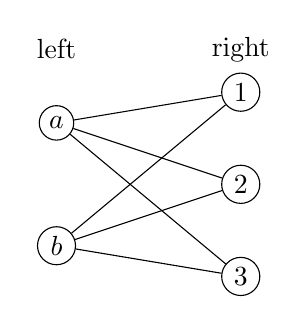
\begin{tikzpicture}[scale=.78,vertex/.style={circle,draw,fill=white,inner sep=2pt}]
\node[vertex] (a) at (0,1) {$a$};
\node[vertex] (b) at (0,-1) {$b$};
\node[vertex] (x) at (3,1.5) {$1$};
\node[vertex] (y) at (3,0) {$2$};
\node[vertex] (z) at (3,-1.5) {$3$};
\foreach \u in {a,b} {\foreach \v in {x,y,z} {\draw (\u)--(\v);}}
\node at (0,2.2) {left};\node at (3,2.2) {right};
\end{tikzpicture}
\column{.47\textwidth}
No edges lie within a side.

This example is $K_{2,3}$: all possible cross-side edges are present.

A triangle cannot be split into two sides in this way.
\end{columns}
\end{frame}


\begin{frame}{The adjacency matrix}
Number the vertices $1,\ldots,n$. Define
\[
 A_{ij}=\begin{cases}1,&\{i,j\}\in E,\\0,&\text{otherwise}.\end{cases}
\]
\begin{columns}[c]
\column{.45\textwidth}\Afig[width=\linewidth]{path-three}
\column{.50\textwidth}
\[
 A(P_3)=\begin{pmatrix}0&1&0\\1&0&1\\0&1&0\end{pmatrix}.
\]
\end{columns}
The matrix is symmetric. Its diagonal is zero.
The sum of row $i$ is the degree of vertex $i$.
\end{frame}

\begin{frame}{Matrix multiplication adds the neighbors' values}
Put a number $x_i$ at each vertex. Then
\[
 (Ax)_i=\sum_{j:\{i,j\}\in E}x_j.
\]
For the path on three vertices,
\[
 \begin{pmatrix}0&1&0\\1&0&1\\0&1&0\end{pmatrix}
 \begin{pmatrix}2\\5\\7\end{pmatrix}
 =\begin{pmatrix}5\\9\\5\end{pmatrix}.
\]
The middle vertex adds $2+7=9$.
The endpoints each see only the middle value, $5$.

This local addition rule is the starting point for both spectral methods
and the exact recovery algorithm later in the talk.
\end{frame}

\begin{frame}{Powers of the adjacency matrix count walks}
The entry $(A^2)_{ij}$ counts walks of length two from $i$ to $j$:
\[
 (A^2)_{ij}=\sum_k A_{ik}A_{kj}.
\]
For $P_3$,
\[
 A^2=\begin{pmatrix}1&0&1\\0&2&0\\1&0&1\end{pmatrix}.
\]
There are two length-two returns from vertex $2$:
$2,1,2$ and $2,3,2$.

More generally, $(A^\ell)_{ij}$ counts length-$\ell$ walks. Induction
works because the last step chooses the final neighbor.
\end{frame}

\begin{frame}{An eigenvector reproduces itself under neighbor addition}
A nonzero vector $x$ is an \emph{eigenvector} with \emph{eigenvalue}
$\lambda$ if $Ax=\lambda x$.
\[
 A(P_3)\begin{pmatrix}1\\\sqrt2\\1\end{pmatrix}
 =\begin{pmatrix}\sqrt2\\2\\\sqrt2\end{pmatrix}
 =\sqrt2\begin{pmatrix}1\\\sqrt2\\1\end{pmatrix}.
\]
The three eigenvalues of $A(P_3)$ are $\sqrt2,0,-\sqrt2$.
For example, $(1,0,-1)^{\mathsf T}$ has eigenvalue zero:
the two contributions at the middle vertex cancel.

For a real symmetric matrix, all eigenvalues are real and an orthonormal
eigenbasis exists: the spectral theorem.
\end{frame}

\begin{frame}{Three visible modes on a cycle}
\begin{center}\Afig[width=.96\textwidth]{cycle-modes}\end{center}
The displayed numbers are vector coordinates, not vertex names.
At every vertex, add the two neighboring numbers.

For $C_4$, the full adjacency spectrum is $2,0,0,-2$.
The second zero mode is $(0,1,0,-1)^{\mathsf T}$.
\end{frame}

\begin{frame}{Regularity produces an exact eigenvector}
If $G$ is $d$-regular, then
\[
 A\one=d\one.
\]
Every row adds exactly $d$ ones.

If $G$ is also bipartite, give one side value $+1$ and the other $-1$.
Every neighbor lies on the opposite side, so
\[
 Ax=-dx.
\]
For example, $C_4$ is $2$-regular and bipartite, explaining its eigenvalues
$2$ and $-2$ without a determinant calculation.

Other eigenvalues describe variations away from these simple modes.
\end{frame}


\section{The Laplacian and partitioning}


\begin{frame}{The graph Laplacian measures local disagreement}
Let $D=\operatorname{diag}(d(1),\ldots,d(n))$. The Laplacian is
\[
 L=D-A,\qquad (Lx)_i=\sum_{j\sim i}(x_i-x_j).
\]
For $P_3$,
\[
 L=\begin{pmatrix}1&-1&0\\-1&2&-1\\0&-1&1\end{pmatrix},\quad
 L\begin{pmatrix}1\\0\\-1\end{pmatrix}
 =\begin{pmatrix}1\\0\\-1\end{pmatrix}.
\]
The constant vector has eigenvalue zero. The full Laplacian spectrum is
$0,1,3$.
\end{frame}

\begin{frame}{The basic energy identity}
For every real vector $x$,
\[
 x^{\mathsf T}Lx=\sum_{\{i,j\}\in E}(x_i-x_j)^2\ge0.
\]
\textbf{Proof.} Each edge contributes $x_i^2+x_j^2$ to
$x^{\mathsf T}Dx$ and $2x_ix_j$ to $x^{\mathsf T}Ax$.
Subtract and sum.

For $P_3$ and $x=(1,0,-1)^{\mathsf T}$,
\[
 x^{\mathsf T}Lx=(1-0)^2+(0-(-1))^2=2.
\]
A small energy means that neighboring vertices usually receive similar
values.
\end{frame}

\begin{frame}{Zero eigenvalues count connected components}
By the energy identity,
\[
 Lx=0\quad\Longleftrightarrow\quad
 x\text{ is constant on every connected component}.
\]
One direction follows because every squared difference must vanish.
The other follows directly from $(Lx)_i=\sum_{j\sim i}(x_i-x_j)$.

Thus
\[
 \dim\ker L=\text{number of connected components}.
\]
For a connected graph, zero is a simple Laplacian eigenvalue.
This is an exact algebraic statement about connectivity.
\end{frame}

\begin{frame}{The second eigenvector is the smoothest nonconstant signal}
For a connected graph, write $0=\lambda_1<\lambda_2\le\cdots\le\lambda_n$.
The spectral theorem gives
\[
 \lambda_2=\min_{x\ne0,\;x\perp\one}
 \frac{\sum_{\{i,j\}\in E}(x_i-x_j)^2}{\sum_i x_i^2}.
\]
A minimizing vector is a \emph{Fiedler vector}.
The orthogonality condition excludes constant signals.

Spectral partitioning orders vertices by this vector, then tests threshold
cuts. A slowly varying signal can expose a weak connection between groups.
The best cut and a balanced cut are not automatically the same thing.
\end{frame}

\begin{frame}{Example: two complete graphs joined by one edge}
\begin{center}\Afig[width=.91\textwidth]{spectral-cut}\end{center}
Here the Fiedler vector has one sign on each $K_4$.
Thresholding at zero finds the single bridge.

For this example, $\lambda_2=3-\sqrt7\approx0.354$.
This illustrates the method; it is not a recovery guarantee for every graph.
\end{frame}

\begin{frame}{A cut gives an upper bound on the second eigenvalue}
In the preceding eight-vertex graph, put $x_i=+1$ on the left $K_4$
and $x_i=-1$ on the right. Then $x\perp\one$.

Only the bridge contributes to the energy:
\[
 x^{\mathsf T}Lx=4,\qquad x^{\mathsf T}x=8,
 \qquad\lambda_2\le\frac48=\frac12.
\]
The actual minimizing vector gives the sharper value $3-\sqrt7$.

This calculation explains why a sparse connection can produce a small
Laplacian eigenvalue.
\end{frame}

\begin{frame}{Keep adjacency and Laplacian eigenvalues distinct}
For a $d$-regular graph, $L=dI-A$. Thus
\[
 Ax=\theta x\quad\Longrightarrow\quad Lx=(d-\theta)x.
\]
For irregular graphs, $D$ is not a scalar matrix, so this conversion
is unavailable.

A \emph{spectral gap} means a specified separation between eigenvalues;
one must say which matrix and which eigenvalues.

The recovery theorem at the end does not require a planted adjacency
eigenvalue to be isolated from the other adjacency eigenvalues.
\end{frame}


\section{Pairings, lifts, and Proposition 28}


\begin{frame}{Pairings between two equal sides are permutations}
\begin{center}\Afig[height=3.55cm,width=.94\textwidth,keepaspectratio]{teaching-bipartite-perfect}\end{center}
A perfect matching pairs every left vertex with a different right vertex.
This one-to-one assignment is a \emph{bijection}, or permutation of the right labels.

The matrix records a $1$ for each selected pair: exactly one $1$ per row and column.
\end{frame}

\begin{frame}{What does a uniformly random perfect matching mean?}
Suppose every left vertex may pair with every right vertex.
For three vertices on each side:
\[
 3\text{ choices for the first partner}\;\times\;
 2\text{ for the next}\;\times\;1=6.
\]
\begin{block}{Uniform means equally likely}
Each of the six complete pairings has probability $1/6$.
For $N$ vertices on each side there are $N!$ pairings, each with probability $1/N!$.
\end{block}
Once a right vertex is paired, no other left vertex may use it.
That restriction makes different matching entries dependent.
\end{frame}

\begin{frame}{A lift replaces one edge by a perfect matching}
\begin{center}\Afig[height=3.55cm,width=.95\textwidth,keepaspectratio]{teaching-elementary-lift}\end{center}
A \emph{fiber} is the group of copies of one original vertex.
For each original edge, pair its two fibers by a perfect matching.
Choose these matchings independently for different original edges.
\end{frame}

\begin{frame}{Example: lifting a four-vertex complete graph}
\begin{center}\Afig[height=3.45cm,width=.83\textwidth,keepaspectratio]{lift-example}\end{center}
Each fiber has two copies. Each original edge contributes one matching.
Every vertex still has three neighbors, one in each other fiber.
\end{frame}


\begin{frame}{Old modes and new modes}
A vector constant on each fiber can be lifted from the base graph.
Neighbor addition on such vectors is exactly the base adjacency action.

Therefore every base eigenvalue is inherited by every lift.
These are the \emph{old} eigenvalues; the orthogonal complement carries
the \emph{new} spectrum.

Bounding the new spectrum requires control of long random walks.
Their products involve entries of the same random matchings, so the
entries cannot be treated as independent.
\source{Bordenave (2020), random-lift spectral theorem and Proposition 28.}
\end{frame}

\begin{frame}{Centering means subtracting the average}
For a random pairing, $M_{ij}$ is $1$ if $i$ is paired with $j$, and $0$ otherwise.
Each of the $N$ possible partners is equally likely, so $\E M_{ij}=1/N$.

Here $\E$ means the average over all possible random pairings.
\begin{example}[A row when $N=3$]
\[
 (0,1,0)\quad\longmapsto\quad
 \left(-\tfrac13,\tfrac23,-\tfrac13\right).
\]
Subtracting the average $1/3$ from every entry makes the row sum zero.
\end{example}
Positive and negative terms can now cancel when we add them.
\end{frame}

\begin{frame}{Centering: a two-cell calculation}
\begin{center}\Afig[width=.65\textwidth]{requested-cells}\end{center}
\[
 \E[(M_{11}-N^{-1})(M_{22}-N^{-1})]
 =\frac1{N(N-1)}-\frac1{N^2}=\frac1{N^2(N-1)}.
\]
In the same row, the expectation is instead $-N^{-2}$.
The dots mark the two entries being averaged, not a complete realized matching.
The position of those entries determines the cancellation.
\end{frame}

\begin{frame}{Prior work and the Proposition 28 question}
\begin{itemize}
\item Bordenave's Proposition 28 bounds products of centered matching entries
in the proof of the random-lift spectral theorem.
\item Brito--Dumitriu--Harris use the same ingredient for bipartite biregular graphs.
\item Collins--Nagatsu give related undepleted recurrences and diagonal leading terms.
\end{itemize}
\begin{block}{Our first contribution}
An intuitive proof: expose compatible pairs, retain the exact remaining
row sum, and use its cancellation before taking absolute values.
\end{block}
The report gives the full product estimate and proof.
\end{frame}

\begin{frame}{After fixing some pairs, the rest are still uniformly paired}
\begin{center}\Afig[height=3.15cm,width=.80\textwidth,keepaspectratio]{depleted-matrix}\end{center}
Two known pairs use two rows and two columns. Four rows and columns remain.

Every perfect matching between these remaining rows and columns is still equally likely.
\begin{block}{Why this helps}
The smaller matching has an exact row sum. Keeping that identity preserves
cancellation that an early absolute-value bound would lose.
\end{block}
\end{frame}

\begin{frame}{How the matching estimate connects to eigenvalues}
\begin{center}
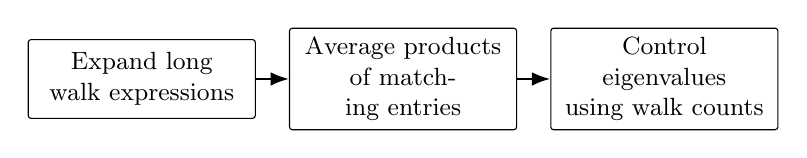
\begin{tikzpicture}[>=Latex,box/.style={draw,rounded corners=1pt,align=center,minimum height=1.0cm,text width=2.65cm,font=\small},node distance=.42cm]
\node[box] (a) {Expand long\\walk expressions};
\node[box,right=of a] (b) {Average products\\of matching entries};
\node[box,right=of b] (c) {Control eigenvalues\\using walk counts};
\draw[->,thick] (a)--(b);\draw[->,thick] (b)--(c);
\end{tikzpicture}
\end{center}
The product estimate supplies the middle step.

The complete graph theorem also needs separate walk-counting and local-cycle estimates.
The report cites those inputs; the product estimate alone is not a new graph spectral theorem.
\end{frame}

\begin{frame}{A half-edge is one end of a future edge}
Attach one small connector, or \emph{half-edge}, for each required neighbor.
Pair one left connector with one right connector to create a full edge.
\begin{center}\Afig[height=3.3cm,width=.96\textwidth,keepaspectratio]{teaching-halfedges}\end{center}
Two left vertices with three connectors each and three right vertices with
two each both supply six connectors. A perfect matching joins the connectors.
This is the idea behind a \emph{biregular} model: one fixed degree on each side.
\end{frame}

% Elementary recovery sequence. The more general theorem and proof details
% belong in the backup slides, rather than this first explanation.
\section{Finding hidden groups}

\begin{frame}{A graph is visible; its group labels are missing}
\begin{center}
\Afig[height=3.9cm]{recovery-uncolored}
\end{center}
The six numbers name the vertices. We see every edge, but no group colors.
\begin{block}{The question}
Can the connections tell us which vertices belong together?
\end{block}
\end{frame}

\begin{frame}{Start with one very concrete neighbor rule}
\begin{columns}[c]
\column{.53\textwidth}
\Afig[height=3.3cm,width=\linewidth,keepaspectratio]{recovery-colored}
\column{.44\textwidth}
Every vertex has:
\begin{itemize}
\item \textbf{two} neighbors in its own group;
\item \textbf{one} neighbor in the other group.
\end{itemize}
These are exact counts, not averages.
\end{columns}
\source{This six-vertex graph illustrates the rule. The theorem later concerns growing random graphs.}
\end{frame}

\begin{frame}{Check the rule at a single vertex}
\begin{columns}[c]
\column{.56\textwidth}
\Afig[height=3.3cm,width=\linewidth,keepaspectratio]{recovery-local-count}
\column{.41\textwidth}
Look at blue vertex \textbf{2}.
\begin{itemize}
\item Vertices 1 and 3 are blue.
\item Vertex 5 is orange.
\end{itemize}
So its counts are
\[
       (\text{same},\text{across})=(2,1).
\]
\end{columns}
A proposed grouping is valid only if \emph{every} vertex passes its rule.
\end{frame}

\begin{frame}{A plausible coloring can fail the rule}
\begin{columns}[c]
\column{.56\textwidth}
\Afig[height=3.3cm,width=\linewidth,keepaspectratio]{recovery-wrong}
\column{.41\textwidth}
In this trial coloring, vertex \textbf{2} has:
\begin{itemize}
\item one neighbor of its own color;
\item two neighbors of the other color.
\end{itemize}
\begin{alertblock}{Reject this trial}
The required counts were $(2,1)$, not $(1,2)$.
\end{alertblock}
\end{columns}
Checking the ordinary neighbor counts gives a definite answer.
\end{frame}

\begin{frame}{The algorithm also tries different count rules}
For a degree-three graph, try tables such as these.
Rows name your group; columns name a neighbor's group.
\begin{columns}[t]
\column{.30\textwidth}
\begin{block}{One group}
\[
\begin{pmatrix}3\end{pmatrix}
\]
Three neighbors inside.
\end{block}
\column{.32\textwidth}
\begin{block}{Two groups}
\[
\begin{pmatrix}2&1\\1&2\end{pmatrix}
\]
Two inside; one across.
\end{block}
\column{.32\textwidth}
\begin{block}{Another rule}
\[
\begin{pmatrix}1&2\\2&1\end{pmatrix}
\]
One inside; two across.
\end{block}
\end{columns}
A fixed upper bound on groups and neighbors leaves only finitely many tables.
The true table is \emph{not} supplied to the algorithm.
\end{frame}

\begin{frame}{The recovery algorithm: five steps}
\begin{center}
\Afig[width=\textwidth]{recovery-workflow}
\end{center}
The hard part is organizing all possible assignments of vertices to groups.

The next slides show how the middle steps work for the specific
\textbf{two-inside, one-across} rule on our six-vertex graph.
\end{frame}

\begin{frame}{Turn a grouping into simple equations}
\begin{columns}[c]
\column{.52\textwidth}
\Afig[height=3.3cm,width=\linewidth,keepaspectratio]{recovery-marks}
\column{.45\textwidth}
Mark group A by $1$ and group B by $0$.
Call the mark at vertex $i$ \,$x_i$.

Adding the neighbors' marks counts neighbors in group A.

At vertex 2 this gives
\[
       x_1+x_3+x_5=1+x_2.
\]
\end{columns}
If $x_2=1$, the count must be 2. If $x_2=0$, it must be 1.
Write one such equation for each vertex and solve them together.
\end{frame}

\begin{frame}{First solve an easier arithmetic version}
\begin{columns}[c]
\column{.53\textwidth}
\Afig[width=\linewidth]{recovery-clock}
\column{.44\textwidth}
Use a three-position clock: after 2 comes 0.

Solve the equations with this arithmetic.
Linear algebra gives a compact description of \emph{all} their solutions.
\end{columns}
Every genuine $0/1$ grouping survives this step, but extra answers can appear.
For example, 1 and 7 look the same on this clock, though they are different integers.
\end{frame}

\begin{frame}{For this graph and this rule: nine clock solutions}
\begin{center}
\Afig[height=3.2cm,width=.96\textwidth,keepaspectratio]{recovery-nine-candidates}
\end{center}
Each boxed string gives the six proposed marks $x_1,\ldots,x_6$.

Seven answers contain a 2, so they are not $0/1$ groupings.
The two remaining answers must still pass the ordinary neighbor-count check.
\source{An exact enumeration of all $3^6$ markings verifies this finite example. It is not the asymptotic theorem.}
\end{frame}

\begin{frame}{Nine candidates become one grouping}
\begin{center}
\Afig[height=3.1cm,width=.92\textwidth,keepaspectratio]{recovery-same-partition}
\end{center}
Both $111000$ and $000111$ pass every ordinary neighbor-count check.
They differ only by exchanging the two group names.
\[
 \boxed{9\text{ clock answers}}\ \longrightarrow\
 \boxed{2\text{ valid colorings}}\ \longrightarrow\
 \boxed{1\text{ division into groups}}.
\]
\source{This count is for the specified $(2,1)$ rule on this particular graph. Other count rules are a separate search.}
\end{frame}

\begin{frame}{Which valid answer should be kept?}
\begin{center}
\Afig[height=3.3cm,width=.96\textwidth,keepaspectratio]{recovery-coarse-fine}
\end{center}
Both pictured answers have a consistent neighbor-count table.
The two-group answer keeps more information than the one-group answer.

The algorithm keeps a valid answer with the most groups, subject to the fixed bound $K$.
\source{These are two illustrative answers; this tiny graph can have other valid groupings. The theorem controls all alternatives in the growing random model.}
\end{frame}

\begin{frame}{Which random graphs does the main case cover?}
\begin{block}{A precise setting, in words}
Every vertex has the same fixed total degree $d\ge3$ and follows a hidden
neighbor-count table with at most $K$ groups.
\end{block}
\begin{itemize}
\item The table connects the groups; their positive size ratios stay fixed.
\item For each group or pair of groups, choose the links uniformly from
all simple graphs with the required counts.
\item These choices are independent.
\end{itemize}
Our example uses random degree-two links inside each group and a random
perfect matching across. Random lifts of fixed regular bases are also covered.
\end{frame}

\begin{frame}{The theorem makes the final choice reliable}
\begin{theorem}[Recovery, stated informally]
In the preceding random model, as the graph grows, with probability tending
to one every valid grouping into at most $K$ groups only merges whole true groups.
\end{theorem}
Therefore the most detailed valid grouping is the hidden one.

The algorithm is given the graph and fixed bounds on groups and degree.
It is \emph{not} given the actual group count, sizes, or neighbor-count table.
\begin{block}{Two separate guarantees}
Every answer on the list passes its exact rules.
Identifying which answer was originally hidden is the high-probability theorem.
\end{block}
\source{The precise statement and complete proofs are in the report's main recovery theorem and proof sections.}
\end{frame}

\begin{frame}{Why is the method computationally useful?}
The proof controls the \emph{average} number of intermediate candidates,
including rare graphs with many of them.

It bounds the expected total work by nearly $n^2$, where $n$ is the number of vertices.
\begin{center}
\Afig[height=2.5cm,width=.75\textwidth,keepaspectratio]{recovery-work-bound}
\end{center}
Doubling $n$ roughly multiplies the bound by four, apart from logarithmic factors.
This is an expected bound, not a speed benchmark or a bound for every input.
\end{frame}

\begin{frame}{What is the new idea, and where does it stop?}
\begin{block}{The useful combination}
Exact neighbor counts give equations. A complete search organized by those
equations can recover unknown groups without needing an isolated signal eigenvalue.
\end{block}
The result covers a broad family of sparse random graphs with fixed parameters,
including every fixed connected simple regular base of degree at least three.
\begin{itemize}
\item The algorithm also learns the count table and group sizes.
\item Exact verification rules out false accepted groupings.
\item Missing or added edges can break the equations: there is no noise theorem here.
\end{itemize}
The formal report proves the model-specific guarantee and explains its predecessors.
\end{frame}


\begin{frame}{What is new, and what came before?}
\begin{block}{The main new result of this report}
A proved recovery guarantee for the stated sparse random models,
with unknown count tables and a proved bound on average computation.
\end{block}
Fellows--Koblitz studied hidden fibers in four-vertex-template covers in 1993.
Bernstein--Cottaar--Lange used Gaussian elimination to expose such fibers in 2023.

The extension is in the proved range and cost guarantee. The algebraic idea
and the classical counting tools have these predecessors.
\source{The report credits prior work and does not certify historical firstness.}
\end{frame}


\begin{frame}{References: background and the matching estimate}
\small
\begin{itemize}
\item B.~Pan, N.~Nie, D.~Wang.
\emph{An Introduction to Spectral Graph Theory}. MIT PRIMES Circle, 2025.
\item C.~Bordenave. \emph{A new proof of Friedman's second eigenvalue theorem
and its extension to random lifts}. Ann. Sci. ENS 53 (2020), 1393--1439.
\item G.~Brito, I.~Dumitriu, K.~D.~Harris.
\emph{Spectral gap in random bipartite biregular graphs and applications}.
CPC 31 (2022), 229--267.
\item B.~Collins, M.~Nagatsu. \emph{Weingarten calculus for centered random
permutation matrices}. Algebraic Combinatorics 9 (2026), 465--479.
\end{itemize}
\end{frame}

\begin{frame}{References and proof locations: recovery}
\small
\begin{itemize}
\item M.~Fellows, N.~Koblitz. \emph{Kid Krypto}. CRYPTO '92 proceedings,
published 1993.
\item D.~J.~Bernstein, J.~Cottaar, T.~Lange. IPCC evaluation, Chapter 3
of \emph{Report on evaluation of KpqC candidates}, 2023, Section 3.1.
\item \emph{Spectral-gap report}: Proposition 28, followed by the main recovery theorems and their complete proofs.
\item \emph{Unknown-frame recovery in sparse block-regular graphs},
November 15, 2026: complete source paper, additional ambiguity,
old/new-spectrum, and information-obstruction results.
\end{itemize}
The full source paper and this talk distinguish proved statements,
cited inputs, internal checks, and historical-priority limits.
\end{frame}

\appendix
\section{Backup: precise statements and calculations}
\begin{frame}{Backup: technical details}
The main talk used a graph example and the equal-degree case.
These optional slides state the broader hypothesis and the algebra behind the algorithm.
\end{frame}


\begin{frame}{Pairing two equal sides gives a permutation matrix}
A uniform permutation $\sigma$ of $\{1,\ldots,N\}$ defines
\[
 M_{ij}=\mathbf 1_{\{\sigma(i)=j\}},\qquad \E M_{ij}=N^{-1}.
\]
Every row and every column has exactly one entry equal to one.

For $r$ prescribed matches in distinct rows and columns,
\[
 \Prob(\text{all occur})=\frac{(N-r)!}{N!}=\frac1{(N)_r},
 \quad (N)_r=N(N-1)\cdots(N-r+1).
\]
Two prescribed matches in the same row cannot both occur.
\end{frame}

\begin{frame}{A row sum gives a positive recurrence}
After $r$ pairs are fixed, $U$ has size $N-r$. Set
$Z_{ij}=NU_{ij}-1$; each remaining row sums to $r$.

Let $\mu_j=\E\prod_{i=1}^j Z_{ii}$, with $\mu_0=1$ and $r+j\le N$.
Multiplying a row sum by $\prod_{i<j}Z_{ii}$ gives
\[
 (N-r-j+1)\mu_j
 =(r+2j-2)\mu_{j-1}+(j-1)\mu_{j-2}.
\]
Omit the final term when $j=1$.

The identity for a used column is
$Z_{ii}Z_{ji}=-Z_{ii}-Z_{ji}-1$.
All recurrence coefficients on the right are nonnegative.
This retains cancellation before any absolute-value estimate.
\source{The report proves the depleted recurrence. At $r=0$, the corresponding recurrence is prior work of Collins--Nagatsu.}
\end{frame}

\begin{frame}{Backup: the centered-product bound}
\small
Each color labels one independent uniformly random matching.
Let $P$ be a product of entries $M_{ij}$ and centered entries $M_{ij}-1/N$,
allowing repeated factors, involving $a$ distinct requested cells.

A \emph{centered singleton} is a cell used exactly once, as $M_{ij}-1/N$.
Let $h$ count such cells that share neither their row nor their column
with another requested cell of the same matching; let $b$ count the others.

For $2\le a\le\sqrt N$,
\[
 |\E P|\le\sqrt e\,2^bN^{-a}
 \left(\frac{\sqrt{a-1}}{\sqrt N-\sqrt{a-1}}\right)^h.
\]
This is the report's scalar mixed-product estimate. Its full proof
appears before the main recovery result.
\end{frame}

\begin{frame}{An equitable partition satisfies an exact matrix equation}
A partition is \emph{equitable} if all vertices of group $i$ have the
same number $Q_{ij}$ of neighbors in group $j$.

Let $J_{vi}=1$ when vertex $v$ belongs to group $i$, and zero otherwise.
Then
\[
 AJ=JQ.
\]
For two groups with internal degree $a$ and cross degree $b$,
\[
 Q=\begin{pmatrix}a&b\\b&a\end{pmatrix},\qquad
 A\tau=(a-b)\tau,
\]
where $\tau$ is $+1$ on one group and $-1$ on the other.
The hidden groups create an exact algebraic signal.
\end{frame}

\begin{frame}{The random model and its sufficient condition}
Fix upper bounds $K$ on the number of groups and $D$ on vertex degree.
The true count table $Q=(d_{ij})$ is fixed, has connected type support,
and has fixed positive size proportions obeying
$N_i d_{ij}=N_j d_{ji}$: cross-edge counts agree from both ends.

Each internal regular graph and each cross biregular graph is sampled
independently and uniformly among simple graphs with those counts.

The theorem requires weights satisfying
\[
 q_{ij}=q_{ji},\qquad 0\le q_{ij}<\tfrac12,\qquad
 \sum_jd_{ij}q_{ij}=1.
\]
The weights certify applicability; the algorithm is not given them.
If all degrees equal $d\ge3$, use $q_{ij}=1/d$.
\end{frame}

\begin{frame}{A complete kernel basis is a certificate of coverage}
If a finite-field solution space has dimension $h$, a basis describes
all its $p^h$ elements using $h$ coefficients in $\F_p$.

The algorithm certifies the \emph{complete} right kernel, even when the
matrix is nonsymmetric. It then enumerates its candidates and verifies
their integer neighbor counts.

Finding one attractive solution would not prove that all valid partitions
had been considered. Completeness is what justifies selecting a finest one.

The randomized computation is always correct; randomness affects its
running time. Such an algorithm is called \emph{Las Vegas}.
\end{frame}

\begin{frame}{Why the expected search cost is nearly quadratic}
The key probabilistic estimate is a \emph{raw moment} bound:
\[
 \sup_n\E\big[p^{h_R(A)}\big]<\infty
\]
for every fixed candidate matrix $R$ and field, where
$h_R(A)=\dim\{Y:AY=YR\}$ over that field.

It counts the average number of modular candidates, including rare
inputs with very large solution spaces.

Combined with the certified sparse computation, it gives expected
$\widetilde O(n^2)$ bit work and expected $\widetilde O(n)$ working bits.
The tilde hides logarithmic factors; fixed-parameter constants may be large.
\end{frame}

\begin{frame}{A sharp ambiguity example from the full research manuscript}
For equal groups of size $N$, internal degree $2$ and cross degree $1$,
choose the hidden balanced grouping uniformly.
\begin{center}\Afig[width=.59\textwidth]{ambiguity-rates}\end{center}
The ambiguity probability is $\sim4/N^2$; the optimal average error is
$\sim2/N^2$. These are asymptotic formulas, not finite-size error bars.
\source{Proved in the full 60-page research manuscript, two-class ambiguity section. This additional result is distinct from the report's condensed core recovery proof.}
\end{frame}

\begin{frame}{Boundary cases show why the assumptions matter}
\textbf{Degree two.} An unconditioned lift of a known cycle is a collection
of cycles. Components admit different shifts and orientations of their
hidden labels. Optimal hidden-fiber success tends to zero.

\textbf{Unequal degrees.} A $K_{3,12}$ lift has exponentially many compatible
fiber partitions, even after the three left fibers are revealed.
Under a uniform remaining hidden prior, optimal success is exponentially small.

Thus minimum degree three by itself does not suffice for arbitrary
nonregular templates. The positive theorem uses the full weight condition.
\source{These separate information bounds are proved in the full research manuscript. Connected conditioning changes the cycle experiment.}
\end{frame}


\end{document}
